\documentclass[12pt]{report}
\usepackage[utf8]{inputenc}
\usepackage[T1]{fontenc}
\usepackage{titlesec}
\usepackage{amsmath}
\usepackage{amsfonts}
\usepackage{amssymb}
\usepackage{enumitem}
\usepackage{bbm}
\usepackage{fancyhdr}
\usepackage{stmaryrd}
\usepackage{listings}
\usepackage{graphicx}
\usepackage{float}
\usepackage{datetime}
\usepackage{textcomp}
\usepackage{color}
\usepackage[colorlinks=true,linkcolor=blue,citecolor=blue, urlcolor=blue]{hyperref}
\usepackage{amsthm}
\usepackage{upgreek}
\usepackage{latexsym}
\usepackage{dirtytalk}
\usepackage{caption}
\usepackage{setspace}
\usepackage{geometry}
\graphicspath{ {images/} }


%\setlength{\parindent}{0pt}
\theoremstyle{definition}
\newtheorem{defi}{Definition}[section]
\newtheorem{thm}[defi]{Theorem}
\newtheorem{corol}[defi]{Corollary}
\newtheorem{lemme}[defi]{Lemma}
\newtheorem{prop}[defi]{Proposition}
\newtheorem*{thm*}{Theorem}

\theoremstyle{remark}
\newtheorem{rem}[defi]{Remark}




\DeclareMathOperator{\argmin}{argmin}
\DeclareMathOperator{\argmax}{argmax}
\DeclareMathOperator{\kl}{KL}
\DeclareMathOperator{\tv}{TV}
\DeclareMathOperator{\data}{data}
\DeclareMathOperator{\lip}{Lip}
\DeclareMathOperator*{\diam}{diam}
\DeclareMathOperator{\tw}{TW}
\DeclareMathOperator{\sgn}{sign}
\DeclareMathOperator{\dom}{dom}
\DeclareMathOperator*{\diag}{diag}
\DeclareMathOperator*{\id}{id}




\begin{document}

%%%%%%%%%%
% Couverture
%%%%%%%%%%
\newgeometry{textwidth=18cm,textheight=24cm,bottom=2cm}
\thispagestyle{empty}
\noindent
\begin{minipage}{0.5\textwidth}
  \begin{flushleft} \Large
    \textsc{Romon} Gabriel\\
    \hfill\\
    \hfill
  \end{flushleft}
\end{minipage}
\noindent
\begin{minipage}{0.5\textwidth}
  \begin{flushright} 
  \Large
    MVA\\
    \textit{Master's Thesis}\\
    \textit{School year 2018-2019}
  \end{flushright}
\end{minipage}

%\vfill
 \vspace*{5cm}

\begin{center}
    \fbox{\parbox{0.9\textwidth}{
        \begin{huge}\begin{center}
            \textbf{Research internship\\ in\\ Optimal Transport}
        \end{center}\end{huge}}}
\end{center}

\vfill
\noindent
\begin{minipage}{0.5\textwidth}
  \begin{flushleft} \Large
    CREST - ENSAE\\
    Palaiseau\\
    \hfill
  \end{flushleft}
\end{minipage}
\noindent
\begin{minipage}{0.5\textwidth}
  \begin{flushright} \Large
    Supervisors : Marco \textsc{Cuturi}\\
    and Victor-Emmanuel \textsc{Brunel}\\
    13/06/2019 - 06/12/2019
  \end{flushright}
\end{minipage} 
%%%%%%%%%%
% Fin couverture
%%%%%%%%%%

\restoregeometry
\newpage\phantom{blabla}

\tableofcontents
\newpage\phantom{blabla}
\onehalfspacing

%%%%%%%%%%
% Introduction
%%%%%%%%%%
\chapter*{Introduction}

\hspace{\parindent}This report summarizes my research internship at CREST, the topic of which was optimal transport. It is an extensive field of research, at the intersection between probability theory, analysis and geometry. The cost of entry into this theory is high, and I spent a considerable amount of time getting up to speed with the basics and browsing the literature.\\
\par This report starts with a self-contained introduction to optimal transport, so that the reader is equipped with enough knowledge to understand the rest. It is followed by an exposition of the internship's research topics: tree metrics, the algorithmic complexity of Sinkhorn's algorithm and the statistical properties of optimal transport.\\
\par Whenever a reference gave a claim without proof, or whenever I found the proof to be lacking in rigor, I chose to write my own. All the proofs in the report are my own work.\\
\par Original contributions are my implementation of the tree-Wasserstein distance, the correction of mistakes in \cite{altschuler2017near} and the Theorem \ref{thmgen}, which is a significant generalization of Theorem 1 in \cite{genevay2018sample}.

%%%%%%%%%%
% Fin introduction
%%%%%%%%%%

\newgeometry{textwidth=16cm, textheight=23cm}
%%%%%%%%%%
% Chapitre 1: intro au transport
%%%%%%%%%%

\onehalfspacing
\chapter{Introduction to Optimal Transport}

\section{Comparing probability measures}

\hspace{\parindent}Comparing probability distributions is a longstanding problem of probability theory that has major implications in the fields of statistics and machine learning. 
\par
From a probabilistic standpoint, the ubiquitous notion of convergence in distribution leads naturally to the study of distances that metrize this convergence \cite{billingsley1971convergence}.  
\par
From a statistical standpoint, these discrepancies can be used to devise statistical tests that determine whether a sample is drawn from a known reference distribution, whether two samples are drawn from the same unknown distribution \cite[Theorem~8.5 and~8.7]{bhattacharya2016course}, \cite{gretton2012kernel} or whether a sample is drawn from either of two reference distributions \cite[Theorem~13.1.1]{lehmann2006testing}. 
\par
From a machine learning standpoint, these concepts are involved whenever one seeks to compare normalized histograms, which are equivalent to discrete probability distributions. In computer vision, an image may be represented by histograms of local features related to color, texture or shape. Comparing the respective histograms of two images indicates whether these images are similar \cite{kolouri2017optimal}. In natural language processing, a document may be viewed as a bag-of-words, i.e.\ as a histogram over the vocabulary, and this provides a natural notion of distance between documents \cite{kusner2015word}. In generative modelling, one may be interested in fitting the unknown data-generating distribution with a parametric distribution. The notion of fit depends intrinsically on the way of comparing the distributions.
\newpage
Let $(\Omega,\mathcal A)$ be a measurable space and $P,Q$ be probability measures on that space. A classical way of comparing $P$ and $Q$ is via \textbf{$f$-divergences}.

\begin{defi}
	Let $f:\mathbb R\to \mathbb R$ be a convex function such that $f(1)=0$. Standard results on slopes of convex functions imply that the limit $f'_\infty:= \lim_{x\to\infty} \frac{f(x)}x$ exists in $\mathbb R\cup \{\infty\}$. By Lebesgue's decomposition theorem \cite[Theorem~7.33]{klenke2013probability},\\ $P$ writes uniquely as $P_a+P_s$ where $P_a,P_s$ are finite non-negative measures such that $P_a\ll Q$ and $P_s\perp Q$.
	The $f$-divergence between $P$ and $Q$ is defined by $$D_f(P\|Q) := \int_\Omega f\left(\frac{dP_a}{dQ}(w) \right) dQ(w) + f'_\infty P_s(\Omega)$$
\end{defi}

Here are examples of well-known divergences. With $f:t\mapsto t\log t$ and $f:t\mapsto (t-1)^2$ one recovers respectively the \textbf{Kullback-Leibler} and the $\mathbf{\chi^2}$ divergences. In both cases, $f'_\infty=\infty$, so theses divergences blow up whenever $P$ is not dominated by $Q$. The functions $f:t\mapsto \frac 12 |t -1|$ and $f:t\mapsto (\sqrt t -1)^2$ define respectively the \textbf{total variation} and \textbf{squared Hellinger} divergences. For these divergences, $f'_\infty<\infty$ and $D_f(P\|Q)$ remains finite for any $P,Q$.

\begin{thm}
	1. $D_f(P\|Q)$ is well-defined, $D_f(P\|Q)\geq 0$ and $D_f(P\|P)=0$.\\
	2. If $f$ is strictly convex, $D_f(P\|Q)=0 \implies P=Q$.
\end{thm}

\begin{proof}
	1. Write $P=P_a + P_s$ the Lebesgue decomposition of $P$ with respect to $Q$. Since $f$ is convex, Theorem 7.9 in \cite{klenke2013probability} implies that $\int_\Omega f\left(\frac{dP_a}{dQ}(w) \right)^- dQ(w)<\infty$, so the integral in the definition is well-defined (although potentially equal to $+\infty$) and additionally $\int_\Omega f\left(\frac{dP_a}{dQ}(w) \right) dQ(w)\geq f\left(\int_\Omega \frac{dP_a}{dQ}(w) dQ(w) \right) = f(P_a(\Omega))$.\\
	For $x\in \mathbb R$, the function $z\mapsto \frac{f(z)-f(x)}{z-x}$ is non-decreasing and bounded above by $f'_\infty$, thus for $y>0$ and $z=x+y$, one gets $\frac{f(x+y)-f(x)}{y}\leq f'_\infty$, that is $f(x) + f'_\infty y \geq f(x+y)$.\\
	By the previous bound, $\begin{aligned}[t] D(P||Q)&\geq f(P_a(\Omega)) + f'_\infty P_s(\Omega)\\
	&\geq f(P_a(\Omega) + P_s(\Omega)) = f(P(\Omega))=f(1)=0\end{aligned}$ \\
	The decomposition of $P$ with respect to itself is $P=P+0$, so that $D(P\|P)=0$.\\
	2. If $D_f(P\|Q)=0$, equality is attained in Jensen's inequality. Since $f$ is strictly convex, there is some constant $C$ such that $\frac{dP_a}{dQ} = C$ $Q$-almost everywhere. By the definition of density we have $\forall A\in \mathcal A, P_a(A) = C Q(A)$ and since $Q(\Omega)=1$ we get $C=P_a(\Omega)$.\\
	Since $f$ is strictly convex, the slope inequality is strict: $\forall y> 0, f(x) + f'_\infty y > f(x+y)$. $D_f(P\|Q)=0$ implies that $P_s(\Omega)=0$, hence $P_s=0$, $P=P_a$, $P_a(\Omega)=1$ and $P=Q$. 
\end{proof}
\newpage 
In general, $f$-divergences are not distances on the space of probability measures. Indeed they have no reason to be symmetric or to verify the triangle inequality. Remarkably, the total variation and Hellinger discrepancies turn out to be distances.
\begin{rem}
 	The terms \say{distance} and \say{metric} carry the same meaning in this report.
\end{rem} 
%mention metrization of weak convergence ?

\par
Suppose $(\Omega,\mathcal A)=(X,\mathcal B(X))$ where $(X,d)$ is a metric space and $\mathcal B(X)$ denotes the Borel $\sigma$-algebra of $X$. The $f$-divergences defined above make no use of the metric $d$ to compare probability measures on $X$. Therefore, one may level the criticism that $f$-divergences overlook geometric properties of $X$. This is clear when one considers two points $x,y\in X$ and the associated Dirac measures $\delta_x$ and $\delta_y$. When $x\neq y$, the values of $D_f(\delta_x, \delta_y)$ for different $f$ are displayed in Table~\ref{tab:1}. 

\begin{center}
\begin{tabular}{|c||c|c|c|c|} \hline
$f$ &  Kullback-Leibler & $\chi^2$ & Total variation & Squared Hellinger \\ \hline
$D_f(\delta_x\|\delta_y)$ &
\begin{tabular}{c} $\infty$
\end{tabular} &
\begin{tabular}{c} $\infty$
\end{tabular} &
\begin{tabular}{c} $1$
\end{tabular} &
\begin{tabular}{c} $2$
\end{tabular}  \\ \hline
\end{tabular}
\captionof{table}{Values of $D_f(\delta_x\|\delta_y)$ for different $f$, with $x\neq y$ \label{tab:1}}
\end{center}

\begin{proof}
	When $x\neq y$, $\delta_x$ and $\delta_y$ have disjoint supports so $\delta_x$ is not dominated by $\delta_y$, hence $\kl(\delta_x\|\delta_y)=\chi^2(\delta_x\|\delta_y)=\infty$. It is well-known \cite[Section~2.4]{tsybakov2004introduction} that the total variation can be rewritten as $\tv(P\|Q)=\sup_{A\in \mathcal B(X)} |P(A)-Q(A)|$ and the squared Hellinger as $H^2(P\|Q) = 2\left(1-\int_{X} \sqrt{\frac{dP}{d\nu}(z)\frac{dQ}{d\nu}(z)} d\nu(z) \right)$ where $\nu$ is any non-negative measure that dominates both $P$ and $Q$ ($\nu= \frac{P+Q}2$ e.g.). By considering $A=\{x\}$ it is clear that $\tv(\delta_x\|\delta_y)=1$. Let $\nu=\frac 12 \delta_x + \frac 12 \delta_y$ and note that $\delta_x \ll \nu$ and $\delta_y \ll \nu$ with respective densities $z\mapsto 2\cdot 1_{z=x}$ and $z\mapsto 2\cdot 1_{z=y}$, so that \\
	$\int_{X} \sqrt{\frac{d\delta_x}{d\nu}(z)\frac{d\delta_y}{d\nu}(z)} d\nu(z) = \frac 12 \int \sqrt{\frac{d\delta_x}{d\nu}(z)\frac{d\delta_y}{d\nu}(z)} d(\delta_x)(z) + \frac 12 \int \sqrt{\frac{d\delta_x}{d\nu}(z)\frac{d\delta_y}{d\nu}(z)} d(\delta_y)(z)  = 0$ and $H^2(P\|Q)=2$.
\end{proof}

It is reasonable to consider instead discrepancies that compare $\delta_x$ and $\delta_y$ by relying on $d(x,y)$. This is one of the motivations behind optimal transport.


\section{The Kantorovitch problem}

\hspace{\parindent} Let $X$ and $Y$ be two Polish spaces (i.e.\ separable and complete metric spaces) and let $P(X), P(Y)$ denote the space of Borel probability measures on $X$ and $Y$ respectively. Consider $c:X\times Y\to \mathbb R_+\cup \{\infty\}$ a lower semi-continuous \textbf{cost function} and two probability measures $\alpha\in P(X), \beta\in P(Y)$. 

\begin{defi}
	A \textbf{coupling} of $(\alpha,\beta)$ is a probability measure $\pi \in P(X\times Y)$ with marginals $\alpha$ and $\beta$, i.e.\
	$\forall A\in \mathcal B(X), \pi(A\times Y)=\alpha(A)$ and $\forall B\in \mathcal B(Y), \pi(X\times B)=\beta(B)$.\\
	The set of couplings of $(\alpha,\beta)$ will be noted as $\Pi(\alpha, \beta)$. 
\end{defi}

Note that $\Pi(\alpha, \beta)$ is non-empty since it contains the trivial coupling $\alpha \otimes \beta$. \textbf{Kantorovitch's mass transportation problem} compares $\alpha$ and $\beta$ by minimizing a linear functional over $\Pi(\alpha, \beta)$.

\begin{defi}
	Kantorovitch's optimal transportation problem between $\alpha$ and $\beta$ is the following:
	\begin{equation}\tag{KP}\label{KP}
	\inf_{\pi\in \Pi(\alpha, \beta)} \int_{X\times Y} c(x,y) d\pi(x,y)
	\end{equation}
\end{defi}
\hfill\\
This problem has been studied extensively in the last 60 years and the relevant theory is developed in any of the following references \cite{rachev1998mass,villani2003topics,villani2008optimal,santambrogio2015optimal}.\\
~\eqref{KP} admits the following dual formulation. 

\begin{thm}
	Let $\Phi_c$ be the set of potentials $(\varphi, \psi)\in L^1(\alpha)\times L^1(\beta)$ such that\\ $\varphi(x)+\psi(y)\leq c(x,y)$ for $\alpha$-almost all $x$ and $\beta$-almost all $y$. Then
	\begin{equation}\tag{KP-dual}\label{KPdual}
	\inf_{\pi\in \Pi(\alpha, \beta)} \int_{X\times Y} c(x,y) d\pi(x,y) = \sup_{(\varphi, \psi)\in \Phi_c} \int \varphi(x) d\alpha(x) + \int \psi(y) d\beta(y)
	\end{equation}
	Besides, the infimum in the LHS is attained and the supremum in the RHS can be restrained to potentials in $C_b(X)\times C_b(Y)$ (i.e continuous and bounded potentials, instead of just integrable).
\end{thm}

\begin{proof}
	See Theorem 1.3 in \cite{villani2003topics}.
\end{proof}

\begin{prop}\label{diracs}
	When $\alpha=\delta_x$ and  $\beta=\delta_y$, the only coupling of $(\alpha,\beta)$ is $\delta_x\otimes \delta_y$ and the value of~\eqref{KP} is $c(x,y)$.
\end{prop}

\begin{proof}
	Let us prove that $\Pi(\delta_x, \delta_y)=\{\delta_x\otimes \delta_y\}$. Consider $\pi\in \Pi(\delta_x, \delta_y)$. Since the products of Borel sets form a pi-system, it suffices to check that \begin{center}$\forall (A,B)\in \mathcal B(X)\times \mathcal B(Y), \pi(A\times B)=\delta_x\otimes \delta_y(A\times B)=\delta_x(A) \delta_y(B)$\end{center}
	When $x\notin A$ or $y\notin B$, since $\pi(A\times B)\leq \pi(A\times Y) = \delta_x(A)$ and $\pi(A\times B)\leq \pi(X\times B) = \delta_y(B)$, we have $\pi(A\times B) \leq \min(\delta_x(A),\delta_y(B))= 0$, hence $\pi(A\times B) = 0 = \delta_x(A) \delta_y(B)$.\\
	When $x\in A$ and $y\in B$, we have $\begin{aligned}[t] 1-\pi(A\times B) &= \pi((A\times B)^c) 
	= \pi((A^c\times Y)\cup (X\times B^c))\\
	&\leq \pi(A^c\times Y) + \pi(X\times B^c)\\
	&= \delta_x(A^c) + \delta_y(B^c)
	= 0
	\end{aligned}$
	Hence $\pi(A\times B)=1=\delta_x(A) \delta_y(B)$\\
	This proves $\pi=\delta_x\otimes \delta_y$ hence $\Pi(\delta_x, \delta_y)=\{\delta_x\otimes \delta_y\}$.
	Since there is only one coupling,~\eqref{KP} is trivial and its minimum is $\int_{X\times Y} c(z)d(\delta_x\otimes \delta_y)(z) = c(x,y)$.
\end{proof}


\section{Wasserstein distances}
%Mention link between OT and total variation

\hspace{\parindent} Suppose $X=Y$, $d$ is a metric on $X$, $p\geq 1$, and consider the cost function \\$c(x,y):=d(x,y)^p$. In this setting,~\eqref{KP} has additional interesting properties.

\begin{defi}
	Let $(X,d)$ be a Polish space, $p\geq 1$ and $\alpha,\beta \in P(X)$.\\ The $p$-\textbf{Wasserstein distance} between $\alpha$ and $\beta$ is defined by 
	\begin{equation}\tag{$p$-Wasserstein}\label{Wp}
	W_p(\alpha, \beta):= \left(\inf_{\pi\in \Pi(\alpha, \beta)} \int_{X\times X} d(x,y)^p d\pi(x,y)\right)^{1/p}
	\end{equation}
\end{defi}

\begin{thm}
	Let $P_p(X)=\{\mu\in P(X)| \; \forall x_0\in X, \int_X d(x,x_0)^p d\mu(x) <\infty \}$ denote the space of probability measures with finite moment of order $p$.\\ Then $W_p$ defines a metric on $P_p(X)$.
\end{thm}

\begin{proof}
	See Theorem 7.3 in \cite{villani2003topics}.
\end{proof}

\begin{rem}
	$W_p$ satisfies the axioms of a metric on $P(X)$. The only issue is that it can be equal to $\infty$. Restricting it to $P_p(X)$ simply ensures that it remains finite. Indeed, if $\alpha, \beta\in P_p(X)$, $\begin{aligned}[t]W_p^p(\alpha, \beta)
	&\leq \int_{X\times X} d(x,y)^p d(\alpha\otimes \beta)(x,y)\\
	&\leq \int_{X\times X} 2^{p-1}(d(x,x_0)^p+d(y,x_0)^p) d(\alpha\otimes \beta)(x,y)\\
	&= 2^{p-1} \left(\int_X d(x,x_0)^p d\alpha(x) + \int_X d(y,x_0)^p d\beta(y) \right) < \infty
	\end{aligned}
	$
\end{rem}
\hfill\\
\par
When $p=1$, duality takes a very simple form.

\begin{thm}\label{1w}
	Let $\mathcal \lip_d=\{\varphi:X\to \mathbb R|\; \forall (x,y)\in X^2, |\varphi(x)-\varphi(y)|\leq d(x,y)\}$ be the set of $1$-Lipschitz functions.
	For $\alpha, \beta\in P_1(X)$, 
	\begin{center}
	$\displaystyle W_1(\alpha, \beta)= \sup_{\varphi \in \lip_d} \int_X \varphi(x) d\alpha(x) - \int_X \varphi(x) d\beta(x)$
	\end{center}
\end{thm}

\begin{proof}
	See Remark 6.5 in \cite{villani2008optimal}.
\end{proof}

The following proposition makes the connection between the total variation distance introduced in Section 1.1 and some Wasserstein distance.
\begin{prop}
	Let $d:(x,y)\mapsto 1_{x\neq y}$ be the trivial metric. Then the associated $1$-Wasserstein is the total variation distance.
\end{prop}

\begin{proof}
	It is clear that for this metric, $P_1(X)=P(X)$.
	It is also well-known \cite[Section~2.4]{tsybakov2004introduction} that $\tv(\alpha\|\beta) = \sup_{A\in \mathcal B(X)} |\alpha(A)-\beta(A)| = \frac 12 \int_X \left|\frac{d\alpha}{d\nu}(x)-\frac{d\beta}{d\nu}(x) \right| d\nu(x)$ where $\nu$ is any non-negative measure that dominates $\alpha$ and $\beta$ ($\nu= \frac{\alpha+\beta}2$ e.g.).\\
	In Theorem \ref{1w}, by considering $-\varphi$ one easily sees that \begin{center}
		$\displaystyle W_1(\alpha, \beta)= \sup_{\varphi \in \lip_d} \left|\int_X \varphi(x) d\alpha(x) - \int_X \varphi(x) d\beta(x)\right|$
	\end{center}
	Let $A\in \mathcal B(X)$. The function $x\mapsto 1_A(x)$ is in $\mathcal L_d$ thus $|\alpha(A)-\beta(A)|=\left|\int 1_A d\alpha-\int 1_A d\beta \right|\leq W_1(\alpha, \beta)$. Taking the supremum over $A$ yields $\tv(\alpha\|\beta)\leq W_1(\alpha, \beta)$.\\
	For the reverse inequality, consider $\varphi\in \lip_d$. The Lipschitz constraint is equivalent to $\forall x,y\in X, |\varphi(x)-\varphi(y)|\leq 1$. One can replace $\varphi$ by $\varphi-c$ (this leaves $\int \varphi d\alpha - \int \varphi d\beta$ untouched and $\varphi$ is still in $\lip_d$) and for a suitable $c$ we can suppose WLOG that $\|\varphi\|_\infty \leq \frac 12$. Let $\nu= \frac{\alpha+\beta}2$ and note that 
	$\begin{aligned}[t] \left|\int_X \varphi(x) d\alpha(x) - \int_X \varphi(x) d\beta(x)\right|
	&\leq \int_X |\varphi(x)| \left|\frac{d\alpha}{d\nu}(x)-\frac{d\beta}{d\nu}(x) \right| d\nu(x)\\
	&\leq \frac 12 \int_X \left|\frac{d\alpha}{d\nu}(x)-\frac{d\beta}{d\nu}(x) \right| d\nu(x)\\
	&= \tv(\alpha\|\beta)
	 \end{aligned}$
	Taking the supremum over $\varphi$ finishes the proof.
\end{proof}

$(P_p(X), W_p)$ has interesting topological properties. Before stating these properties we need to define \textbf{weak convergence} of a sequence in $P(X)$. This is related to convergence in distribution.

\begin{defi}
	Let $(\alpha_n)_n\in P(X)^{\mathbb N}$ and $\alpha \in P(X)$. $(\alpha_n)_n$ converges weakly to $\alpha$ (denoted $\alpha_n \Rightarrow \alpha$) if for every bounded continuous function $f$, \begin{center}$\displaystyle \lim_{n\to \infty} \int_X f(x) d\alpha_n(x) = \int_X f(x) d\alpha(x)$ \end{center}
\end{defi}

\begin{rem}
	Let $(Y_n)_n$ be a sequence of random elements from $(\Omega,\mathcal A,P)$ to $(X,\mathcal B(X))$. $Y_n$ converges in distribution to a random element $Y$ if and only the sequence of image measures $(P_{Y_n})_n$ converges weakly to $P_Y$ (formally, $P_{Y_n}$ is the pushforward of $P$ by $Y_n$). 
\end{rem}

\begin{rem}
	The well-known Portmanteau theorem \cite[Theorem~13.16]{klenke2013probability} provides equivalent conditions for weak convergence.
\end{rem}

A desirable property for any metric $D$ on $P(X)$ is that it \textbf{metrizes} weak convergence, i.e.\ $\alpha_n \Rightarrow \alpha \iff D(\alpha_n, \alpha) \xrightarrow[n\to \infty]{} 0$. Remarkably, the total variation and Hellinger distances define the same topology, and they do not metrize weak convergence. Returning to the example of Dirac measures, consider $X=\mathbb R$, $\alpha_n=\delta_{1/n}$ and $\alpha=\delta_0$. It is clear that $\alpha_n \Rightarrow \alpha$. We proved earlier that $\tv(\alpha_n\|\alpha)=1$, $H^2(\alpha_n\| \alpha)=2$ and by Proposition \ref{diracs} $W_p(\alpha_n,\alpha)=d(\frac 1n, 0)^p$. This suggests that Wasserstein distances have nicer properties, and this is confirmed in the next theorem.

\begin{thm}
 	Let $(\alpha_n)_n\in P_p(X)^{\mathbb N}$ and $\alpha \in P_p(X)$. The following statements are equivalent:
 	\begin{enumerate}[nosep]
 		\item $W_p(\alpha_n, \alpha) \xrightarrow[]{n\to \infty} 0$
 		\item $\alpha_n \Rightarrow \alpha$ and the moment of order $p$ converges: \begin{center}$\displaystyle \forall x_0\in X, \lim_{n\to \infty} \int_X d(x,x_0)^p d\alpha_n(x) =  \int_X d(x,x_0)^p d\alpha(x)$\end{center}
 		\item $\alpha_n \Rightarrow \alpha$ and the following tightness condition is verified: \begin{center}$\displaystyle \forall x_0\in X, \lim_{R\to \infty} \limsup_{n\to \infty} \int_{d(x,x_0)\geq R} d(x,x_0)^p d\alpha_n(x) = 0$\end{center}
 	\end{enumerate}
\end{thm}

\hfill
\begin{proof}
	See Theorem 7.12 in \cite{villani2003topics}.
\end{proof}


\begin{rem}
	When $d$ is bounded or $X$ is bounded, for any $x_0\in X$ the set \\$\{x\in X|\; d(x,x_0)\geq R\}$ is empty for large enough $R$, so that \begin{center}$\displaystyle  \lim_{R\to \infty} \limsup_{n\to \infty} \int_{d(x,x_0)\geq R} d(x,x_0)^p d\alpha_n(x) = 0$\end{center}
	In this bounded case, $P_p(X)=P(X)$ and $W_p$ metrizes weak convergence on the whole of $P(X)$.\\
	In the unbounded case, convergence of moments or the tightness condition need to be checked to infer $W_p(\alpha_n, \alpha) \xrightarrow[]{n\to \infty} 0$.
\end{rem}

\newpage
\section{The discrete case}

\hspace{\parindent} As mentioned in the beginning of Section 1.1, machine learning practitioners often deal with normalized histograms, i.e.\ discrete probability measures. In this section we consider Kantorovitch's problem in the discrete case. A comprehensive reference on this topic is \cite[Chapter~2]{peyre2019computational}.
\\
\par Let $X,Y$ be Polish spaces and $c:X\times Y \to \mathbb R_+$ be a lower semi-continuous cost function. Suppose $\alpha=\sum_{i=1}^n a_i \delta_{x_i}$ and $\beta=\sum_{j=1}^m b_j \delta_{y_j}$ where $n,m\in \mathbb N^*$, $a\in (\mathbb R_+^*)^n$, $b\in (\mathbb R_+^*)^m$ are such that $\sum_{i=1}^n a_i=\sum_{j=1}^m b_j=1$, and $(x_i)_{i\in \llbracket 1,n\rrbracket} \in X^n$, $(y_j)_{j\in \llbracket 1,n\rrbracket} \in Y^m$ are support points. 

\begin{thm}\label{discrete}
	Let $U(a,b)=\{P\in (\mathbb R_+)^{n\times m}|\; P \mathbbm 1_m =a, P^T \mathbbm 1_n =b \}$ denote the convex polytope of matrices with row sums $a$, column sums $b$ and non-negative entries.\\
	In the discrete setting,~\eqref{KP} has the following form:
	\begin{equation*}
	\inf_{P\in U(a,b)} \sum_{i=1}^n\sum_{j=1}^m c(x_i,y_j)P_{ij}
	\end{equation*}
\end{thm}

\begin{proof}
	Given $\pi \in \Pi(\alpha, \beta)$, let us prove that $\pi$ is discrete and supported on the $(x_i,y_j)$ where $(i,j) \in \llbracket 1,n \rrbracket\times \llbracket 1,m \rrbracket$ (note that $\pi(\{(x_i,y_j\})$ may be $0$). It suffices to prove that $\pi([\cup_{i=1}^n \{x_i\}]\times [\cup_{j=1}^m \{y_j\}]=1$, and this is equivalent to \begin{center}$\pi(\left([\cup_{i=1}^n \{x_i\}]^c\times Y\right)\cup \left(X\times [\cup_{j=1}^m \{y_j\}]^c\right))=0$\end{center}
	This holds since \begin{center}
		$\begin{aligned}[t]\pi(\left([\cup_{i=1}^n \{x_i\}]^c\times Y\right)\cup \left(X\times [\cup_{j=1}^m \{y_j\}]^c\right)) &\leq \pi([\cup_{i=1}^n \{x_i\}]^c\times Y) + \pi(X\times [\cup_{j=1}^m \{y_j\}]^c) \\
		& = \alpha([\cup_{i=1}^n \{x_i\}]^c) + \beta([\cup_{j=1}^m \{y_j\}]^c) = 0
		\end{aligned}$
	\end{center}
	Therefore there is some $P\in U(a,b)$ such that $\pi = \sum_{i=1}^n\sum_{j=1}^m P_{ij} \delta_{(x_i,y_j)} $ and the rest of the proof is easy.
\end{proof}

\begin{rem}
	The discrete case boils down to a \textbf{linear programming} problem: the objective and the $n+m$ constraints are linear in $P$.\\
	This problem can be solved exactly with any LP solver, but the best time complexity achieved to date is $O((n+m)nm \log^2(n+m))$ \cite[Section~3.5.3]{peyre2019computational}. When $n=m$ this complexity is $O(n^3\log^2(n))$, whereas the size of the data is $n^2$.
\end{rem}

\chapter{Tree metrics}

\section{Introduction}

\hspace{\parindent} The original goal of the internship was to work on extensions of the following recent paper \cite{le2019tree}, which was accepted at NIPS 2019. The paper considers the $1$-Wasserstein between discrete measures on spaces where the ground metric is a \textbf{tree metric}.

\begin{defi}
	Suppose $(X,d)$ is a metric space and consider a tree $T$ (i.e.\ a connected acyclic undirected graph) whose nodes are elements of $X$. To each edge $e=(z,t)$ in the tree we associate the weight $w_e=d(z,t)$. Given two nodes $z$ and $t$, there is a unique path between them in the tree. $d_T(z,t)$ is defined as the sum of the weights along this path. $d_T$ is called the tree metric associated to $T$.
\end{defi}

\begin{prop}
	$(T,d_T)$ is a metric space.
\end{prop}

\begin{defi}
	Consider $(X,d)$ a metric space, $\alpha=\sum_{i=1}^n a_i \delta_{x_i}$ and $\beta=\sum_{j=1}^m b_j \delta_{y_j}$ discrete measures on $X$. Let $T$ be a tree whose nodes contain the set $\{(x_i)_{i\in \llbracket 1,n\rrbracket}\} \cup \{(y_j)_{j\in \llbracket 1,m\rrbracket}\}$. The \textbf{tree-Wasserstein} between $\alpha$ and $\beta$ is defined as $\tw(\alpha,\beta) := W_1(\alpha,\beta)$ where in the RHS $\alpha,\beta$ are taken as measures on $(T,d_T)$.
\end{defi}

\begin{rem}
	In other words, we embed the original metric space $(X,d)$ into a tree metric space $(T,d_T)$ and we compute the $1$-Wasserstein in the new space.
\end{rem}

It turns out that $\tw(\alpha,\beta)$ has a nice closed form. This owes much to the simplicity of duality for $1$-Wasserstein distances, as seen in Theorem \ref{1w}.

\begin{thm}
	Let $T$ be a tree rooted at an arbitrary $r\in X$ and let $E_T$ denote the set of edges of $T$. For $e\in E_T$, let $u_e$ denote the node closest to the root and $v_e$ the other node (see Figure \ref{schematree}). Additionally, for any node $z\in X$, let $\Gamma(z)$ denote the subtree rooted at $z$. Then 
	\begin{center}
		$\displaystyle \tw(\alpha,\beta) = \sum_{e\in E_T} w_e |\alpha(\Gamma(v_e))-\beta(\Gamma(v_e))|$
	\end{center}
	\begin{figure}[h!]
	\centering
    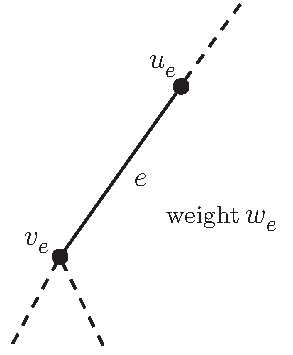
\includegraphics[scale=0.9]{schematree.pdf}
    \caption{An edge $e=(u_e,v_e)$ in a rooted tree}
    \label{schematree}
	\end{figure}
\end{thm}

\begin{proof}
	We make use of the dual form of $1$-Wasserstein. Let $f:T\mapsto \mathbb R$ be $1$-Lipschitz for the metric $d_T$. By replacing $f$ with $f-f(r)$ we can suppose WLOG that $f(r)=0$. For every edge $(u_e,v_e)$ define $\tilde f(v_e):=\frac{f(v_e)-f(u_e)}{w_e}$. Since $f$ is $1$-Lipschitz, $\tilde f$ takes values in $[-1,1]$, and by construction $\displaystyle f(v_e)=\sum_{a\in E_T} 1_{\Gamma(v_a)}(v_e)\tilde f(v_a)w_a$.\\
	Note that $$\begin{aligned}[t]
		\int_T f(t) d\alpha(t) &= f(r)\alpha(\{r\}) + \sum_{e\in E_T} f(v_e)\alpha(\{v_e\}) \\
		&= \sum_{e\in E_T} \sum_{a\in E_T} 1_{\Gamma(v_a)}(v_e)\tilde f(v_a)w_a\alpha(\{v_e\})\\
		&= \sum_{a\in E_T} \tilde f(v_a)w_a \sum_{e\in E_T}  1_{\Gamma(v_a)}(v_e)\alpha(\{v_e\}) \\
		&= \sum_{a\in E_T} \tilde f(v_a)w_a \alpha(\Gamma(v_a))
	\end{aligned}$$
	Hence $$\int_T f(t) d\alpha(t) -\int_T f(t) d\beta(t) = \sum_{e\in E_T} \tilde f(v_e)w_e \left[\alpha(\Gamma(v_e))-\beta(\Gamma(v_e))\right]$$
	The supremum over $f$ is attained for $f^*$ defined recursively by $f^*(r)=0$ and $f^*(v_e)=w_e \sgn(\alpha(\Gamma(v_e))-\beta(\Gamma(v_e)) + f^*(u_e)$. This yields $\tilde f^*(v_e)=\sgn(\alpha(\Gamma(v_e))-\beta(\Gamma(v_e))$, thus 
	$$\tw(\alpha,\beta) = W_1(\alpha,\beta) = \sup_{f\in \lip_{d_T}} \int_T f(t) d\alpha(t) -\int_T f(t) d\beta(t) = \sum_{e\in E_T} w_e |\alpha(\Gamma(v_e))-\beta(\Gamma(v_e))|$$
\end{proof}

\begin{rem}
	Since the proof relies heavily on the dual form of the $1$-Wasserstein, it is very likely that there is no nice closed form for the $p$-Wasserstein on tree metric spaces when $p>1$.
\end{rem}

\section{Personal work}

\hspace{\parindent}
The beginning of the internship was dedicated to implementing the tree-Wasserstein. Note that the authors of \cite{le2019tree} did not release their code, nor did they give pseudo-code for the tree-Wasserstein in their paper.\\
A computational challenge in their approach is that they consider measures $\alpha=\sum_{i=1}^n a_i \delta_{x_i}$ and $\beta=\sum_{j=1}^m b_j \delta_{y_j}$ but the tree $T$ is not given \textit{a priori}. Instead they propose methods to sample trees whose nodes are the support points of the measures. We explored and implemented other methods of sampling using the Python package \verb!NetworkX!.

Assuming $X=\mathbb R^d$, $\alpha=\sum_{i=1}^n a_i \delta_{x_i}$ and $\beta=\sum_{j=1}^m b_j \delta_{y_j}$ we:
	\begin{enumerate}
    \item Generate a connected graph $G$ whose nodes are the support points and whose edges are the Euclidean distances between points. The simplest and fastest way is to use the complete graph on the support points. To get a graph that is sensitive to the geometry of the support points, it is preferable to consider a $k$-NN graph, but it may not be connected. Even if $k$ is reasonably large, if there are two tightly-knit and distant clusters in the support points, it will have at least two components. This can be fixed by adding random edges between the connected components.

    \item Compute a directed spanning tree $T$ on the graph. For our use in tree-Wasserstein, $G$ or $T$ needs to be random.\\
    $\bullet$ BFS and DFS on a connected graph both generate spanning trees. We get random spanning trees simply by randomizing the starting node of the search. An interesting question is the distribution induced by this sampling method on spanning trees of $G$.\\
    $\bullet$ Wilson's algorithm \cite[Theorem~4.1]{lyons2017probability} is based on loop-erased random walks, with transition probabilities proportional to edge weights (or a function thereof). The probability of a spanning tree being sampled is the product of its edge weights.\\
    $\bullet$ Kruskal's or Prim's algorithm can be used to compute a minimum spanning tree, but these are deterministic algorithms (the minimum spanning tree is unique if all the edge weights are distinct).

    \item Prepare $T$ for the computation of $d_{TW}$. Let $T'$ be the tree obtained by reversing the edges in $T$ and compute a topological sort of $T'$. This yields an ordered list of nodes $\ell$. By construction, the leaves of $T$ are the first elements of $\ell$. For each node in $\ell$, add its mass under $\alpha$ and $\beta$ to the corresponding masses of its parent in $T$ (which is its child in $T'$). When this process ends, by construction, the masses at each \verb!node! are $(\alpha(\Gamma(\verb!node!)), \beta(\Gamma(\verb!node!)))$, the masses under $\alpha$ and $\beta$ of the subtree rooted at \verb!node!, which is exactly what we need to compute $\tw$.\\
    As a sanity check, one can verify that the masses affected to the root of $T$ are $(1,1)$.
    \item Compute $d_{TW}$. This is done by simply looping over the edges of $T'$.
    \end{enumerate}

We provide cost analyses for both types of graphs in Table \ref{tab:2} and \ref{tab:3}. Let $N=n+m$ be the number of nodes of the graph. The number of edges in the complete graph is $\frac{N(N-1)}2=\Theta(N^2)$ and $\frac{kN}2=\Theta(kN)$ for the $k$-NN graph.

\begin{table}[H]
\centering
\begin{tabular}{|c|c|c|c|}
  \hline
    \multicolumn{2}{|c|}{Step} & Time complexity & Space complexity\\ \hline 
   Generation & & $\Theta(N^2d)$ & $\Theta(N^2)$\\
   Spanning tree & BFS/DFS & $\Theta(N^2)$ & $O(N)$ \\
    & Wilson & ? & $O(N)$ \\
    Preparation & & $\Theta(N)$ & $O(N)$\\
    TW computation & & $\Theta(N)$ & $\Theta(1)$\\
   \hline
\end{tabular}
\caption{Complexity estimates for a complete graph \label{tab:2}}
\end{table}

\begin{table}[H]
\centering
\begin{tabular}{|c|c|c|c|}
  \hline
    \multicolumn{2}{|c|}{Step} & Time complexity & Space complexity\\ \hline 
   Generation & & ? & $\Theta(kN)$\\
   Spanning tree & BFS/DFS & $\Theta(kN)$ & $O(N)$ \\
    & Wilson & ? & $O(N)$ \\
    Preparation & & $\Theta(N)$ & $O(N)$\\
    TW computation & & $\Theta(N)$ & $\Theta(1)$\\
   \hline
\end{tabular}
\caption{Complexity estimates for a $k$-NN graph \label{tab:3}}
\end{table}

Once the tree is constructed, the time complexity for computing $\tw(\alpha,\beta)$ is $\Theta(n+m)$. This is much better than the $O((n+m)nm \log^2(n+m))$ of LP solvers.
\\
\par The goal of the internship was to adapt the notion of sliced Wasserstein barycenters developed in \cite{bonneel2015sliced} to the tree-Wasserstein. As explained above, trees depend on the measures $\alpha$ and $\beta$ because the support points must be contained in their nodes. On the contrary, sliced Wasserstein is based on sampling random lines in $\mathbb R^d$ and projecting the support points on those lines (so the lines are independent of $\alpha$ and $\beta$). Because of this significant difference, I was not able to come up with a notion of tree-sliced Wasserstein barycenters. Such a notion was recently proposed in \cite{le2019scalable}, but I have not had time to look into it.
\\
\par Given a ground metric $d$, two discrete measures $\alpha, \beta$ and a tree $T$, the authors of \cite{le2019tree} do not study the link between $\tw(\alpha,\beta)$ and $W_1(\alpha,\beta)$. If the tree $T$ is sufficiently well-chosen, we expect that $\tw(\alpha,\beta)$ is not too far from the true $1$-Wasserstein.
\par The identity mapping $\id: (X,d)\to (T,d_T)$ is a \textbf{metric embedding}. We define the expansion of $\id$ as $\sup_{x\neq y\in X} \frac{d_T(x,y)}{d(x,y)}$, its contraction as $\sup_{x\neq y\in X} \frac{d(x,y)}{d_T(x,y)}$ and its distortion as the product of the expansion and the contraction. Equivalently, the distortion of $\id$ is the minimum $\lambda\geq 1$ such that \begin{center}
	$\exists\mu>0, \forall (x,y)\in X, \mu d_T(x,y)\leq d(x,y) \leq \lambda \mu d_T(x,y)$
\end{center}
A desirable tree is a $T$ such that $\id$ has low distortion. It is not always possible to construct such a tree: in \cite{rabinovich1998lower} it is proven that any embedding of the $n$-point cycle $C_n$ into a tree metric has distortion at least $\frac n3 -1$. \textbf{Probabilistic embeddings} are a possible workaround \cite{Bartal19}. The paper \cite{fakcharoenphol2004tight} provides a way of sampling trees with distortion $O(\log n)$ (sometimes referred to as FRT trees because of the author's initials).
\par When browsing the literature on tree metrics, I noticed that the paper \cite{leeb2018approximating} makes the connection between FRT trees and the approximation of $W_1(\alpha,\beta)$ by $\tw(\alpha,\beta)$. Numerical experiments carried out on the MNIST dataset show that both quantities are not far from each other (see Figure \ref{leeb})

\begin{figure}[h!]
\centering
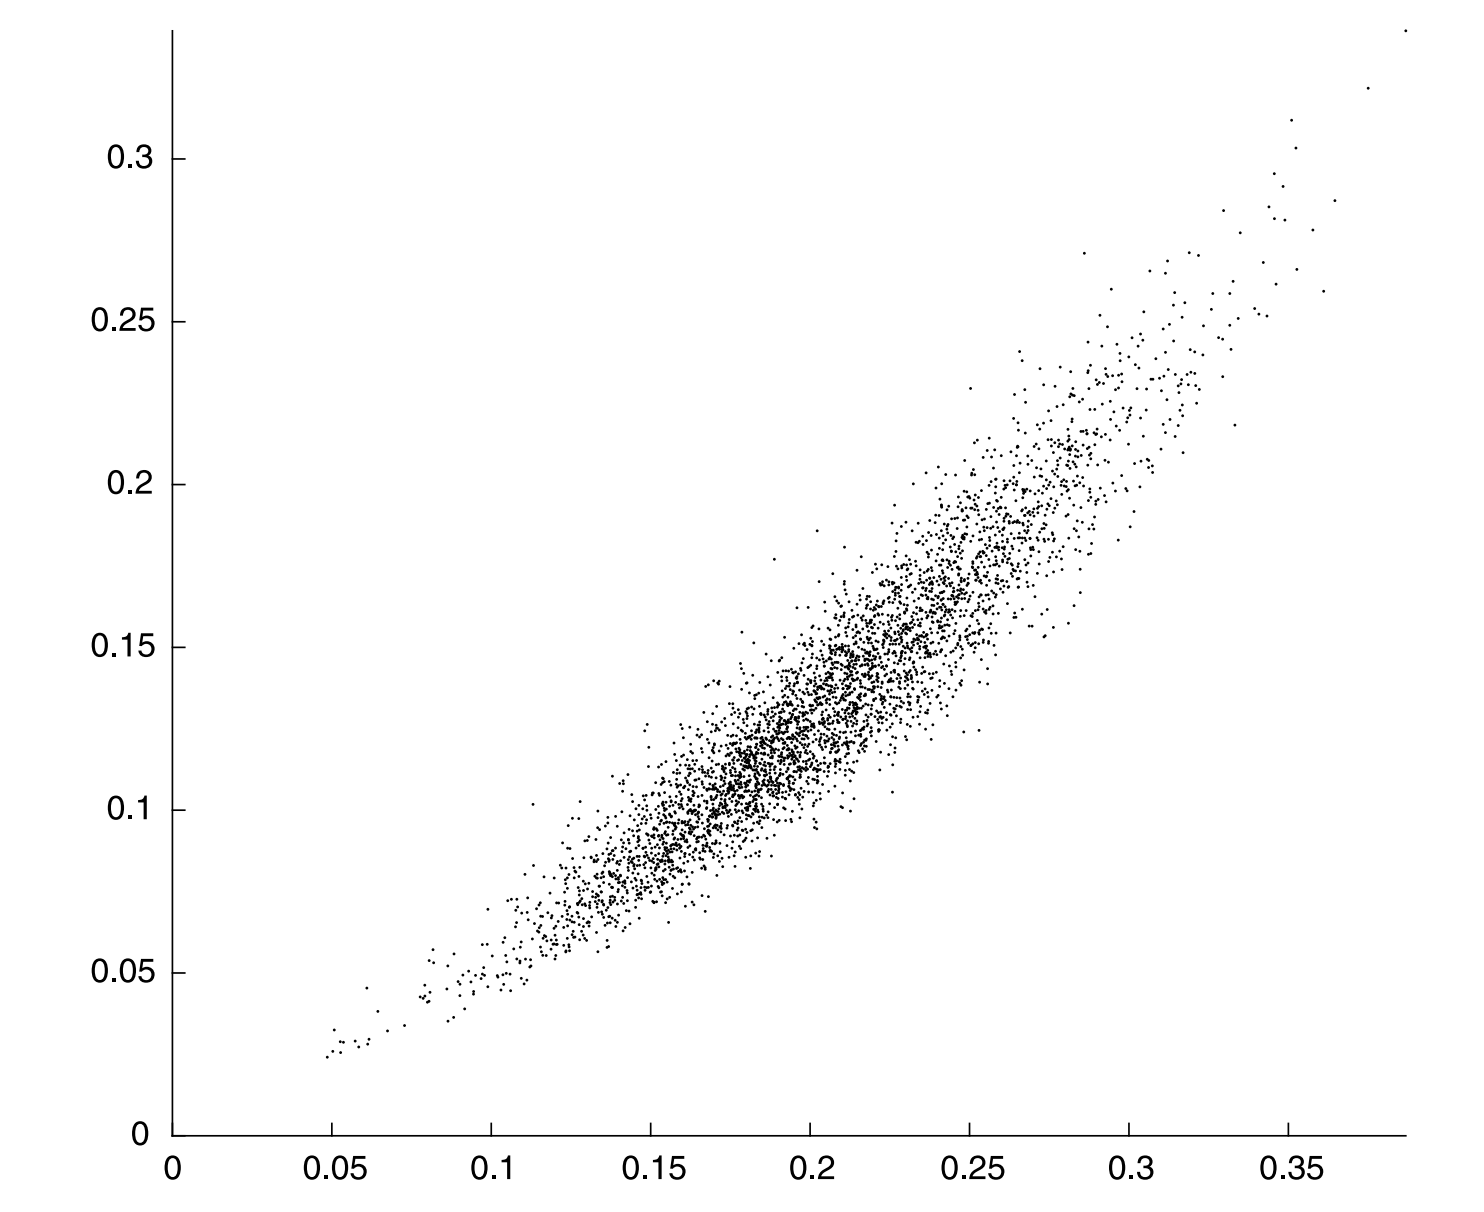
\includegraphics[scale=0.3]{leeb}
\caption{True $W_1$ versus approximate $W_1$, using 25 trees, from \cite{leeb2018approximating}}
\label{leeb}
\end{figure}

\chapter{Regularized Optimal Transport}

\section{Introduction}

\hspace{\parindent} In the discrete case, regularizing Kantorovitch's problem with an entropic term enables the use of an elementary iterative scheme that converges quickly to the minimum. This regularization and the iterative method were introduced in \cite{cuturi2013sinkhorn}.
\\
\par
In the general case, the regularized Kantorovitch's problem is defined using the Kullback-Leibler divergence (already introduced in Section 1.1). Let $(\Omega,\mathcal A)$ be a measurable space and $P,Q$ be probability measures on that space. We define $$\kl(P\|Q):= \begin{cases}
	\int_\Omega \log\left(\frac{dP}{dQ}(w) \right) dP(w) &\text{if } P\ll Q\\
	\infty &\text{otherwise }
\end{cases}$$
If $P\ll Q$, this rewrites as $\int_\Omega \log\left(\frac{dP}{dQ}(w) \right) \frac{dP}{dQ}(w) dQ(w)$ and this is consistent with the definition via $f$-divergences (with $f:x\mapsto x\log x$).

\begin{defi}
	Let $X$,$Y$ be Polish spaces, $c:X\times Y\to \mathbb R_+\cup \{\infty\}$ a lower semi-continuous cost function and two probability measures $\alpha\in P(X), \beta\in P(Y)$. The regularized Kantorovitch's problem is the following.\\
	Given $\varepsilon>0$ a regularization parameter, we consider 
	\begin{equation}\tag{Regularized KP}\label{rKP}
	\inf_{\pi\in \Pi(\alpha, \beta)} \int_{X\times Y} c(x,y) d\pi(x,y) + \varepsilon\kl(\pi\|\alpha\otimes \beta)
	\end{equation}
\end{defi}

\begin{rem}
	The term $\kl(\pi\|\alpha\otimes \beta)$ in the objective forces the transportation plans $\pi$ to be absolutely continuous with respect to $\alpha\otimes \beta$. In general a coupling $\pi\in \Pi(\alpha,\beta)$ need not be dominated by $\alpha\otimes \beta$ (consider $\pi$ the uniform distribution on the diagonal of the unit rectangle $[0,1]\times [0,1]$ and $\alpha$, $\beta$ having $\mathcal U([0,1])$ distribution).
\end{rem}

The regularized problem also admits a dual formulation. A version of the dual problem was first stated in \cite{genevay2016stochastic}, without proof. A proof was added in \cite[Proposition~4]{genevay2019entropy} but it is purely formal and not rigorous. The recent paper \cite{clason2019entropic} provides an in-depth study of duality in the setting where $X=\mathbb R^d$ and the regularization is modified:
	\begin{equation*}
	\inf_{\pi\in \Pi(\alpha, \beta)} \int_{X\times Y} c(x,y) d\pi(x,y) + \varepsilon\kl(\pi\|\lambda_d\otimes \lambda_d)
	\end{equation*}
The authors make heavy use of functional analysis and I plan on spending time on this paper in the coming weeks. In \cite{genevay2016stochastic,genevay2018sample,genevay2019entropy}, duality is stated as follows:

\begin{prop}
	Let $X,Y$ be arbitrary metric spaces, and let $\mathcal C(X)$, $\mathcal C(Y)$ denote the spaces of continuous functions with real values. The convex dual of (\ref{rKP}) is 
	\begin{equation*}\tag{Dual Reg. KP 1}\label{dualrKP}
		\sup_{\substack{\varphi \in \mathcal C(X)\\\psi \in \mathcal C(Y)}} \int_X \varphi(x) d\alpha(x) + \int_Y \psi(y) d\beta(y) -\varepsilon \int_{X\times Y} e^{\frac{\varphi(x)+\psi(y)-c(x,y)}\varepsilon} d(\alpha\otimes\beta)(x,y) + \varepsilon
	\end{equation*}
\end{prop}

In the recent paper \cite{mena2019statistical}, it is stated as follows:

\begin{prop}
	When $X=Y=\mathbb R^d$ and $c:(x,y)\mapsto \|x-y\|_2^2$, the dual of (\ref{rKP}) is 
	\begin{equation*}\tag{Dual Reg. KP 2}\label{dualrKP2}
		\sup_{\substack{\varphi \in L^1(\alpha)\\\psi \in L^1(\beta)}} \int_{\mathbb R^d} \varphi(x) d\alpha(x) + \int_{\mathbb R^d} \psi(y) d\beta(y) -\varepsilon \int_{\mathbb R^d\times \mathbb R^d} e^{\frac{\varphi(x)+\psi(y)-\|x-y\|_2^2}\varepsilon} d(\alpha\otimes\beta)(x,y) + \varepsilon
	\end{equation*}
\end{prop}

The space in which the dual is optimized certainly depends on the regularity of $X,Y, \alpha, \beta$. By the best of our knowledge, there is no result on this dependence in the literature. I plan on studying this issue in the coming weeks, as this is important for the work carried out in Chapter 3.

\newpage
\section{The discrete case}

\begin{prop}\label{discretereg}
	In the discrete case where $\alpha=\sum_{i=1}^n a_i \delta_{x_i}$ and $\beta=\sum_{j=1}^m b_j \delta_{y_j}$ with $n,m\in \mathbb N^*$, $a\in (\mathbb R_+^*)^n$, $b\in (\mathbb R_+^*)^m$, the regularized problem writes as \begin{equation*}
	\inf_{P\in U(a,b)} \sum_{i=1}^n\sum_{j=1}^m c(x_i,y_j)P_{ij} + \varepsilon \sum_{i=1}^n\sum_{j=1}^m P_{ij}\log\left(\frac{P_{ij}}{a_i b_j} \right)
	\end{equation*}
\end{prop}

\begin{proof}
	The proof is similar to that of Theorem \ref{discrete}. It suffices to notice that\\ $\displaystyle \frac{d\pi}{d\alpha\otimes \beta}(x,y)=\sum_{i=1}^n\sum_{j=1}^m \frac{P_{ij}}{a_i b_j} 1_{x=x_i}1_{y=y_j}$.
\end{proof}

\begin{thm}
	The dual formulation for the discrete regularized problem is 
	\begin{center}
		$\displaystyle \sup_{\substack{\lambda\in \mathbb R^n\\ \mu\in \mathbb R^m}} \sum_{i=1}^n \lambda_i a_i+\sum_{j=1}^m \mu_j b_j - \varepsilon \sum_{i=1}^n\sum_{j=1}^m a_i b_j \exp\left(\frac{\lambda_i+\mu_j-c(x_i,y_j)}{\varepsilon}\right) + \varepsilon$
	\end{center}
\end{thm}

\begin{proof}
	Let $g$ denote the objective function in Proposition \ref{discretereg}. $g$ is strictly convex with domain $\dom g=(\mathbb R_+)^{n\times m}$, $g$ is continuous on $\dom g$, and coercive. The constraint set is compact, thus the infimum is actually a minimum, and there is a unique solution.\\
	Since there are only two equality constraints that are linear in $P$, strong duality holds. Let \\$L(P,\lambda,\mu)=\sum_{i=1}^n\sum_{j=1}^m c(x_i,y_j)P_{ij} + \varepsilon \sum_{i=1}^n\sum_{j=1}^m P_{ij}\log\left(\frac{P_{ij}}{a_i b_j} \right) - \lambda^T(P\mathbbm 1_m-a) - \mu^T(P^T \mathbbm 1_n -b)$ be the Lagrange function. For fixed $\lambda, \mu$, $L$ is convex in $P$ and $P_{ij}^* =a_i b_j \exp\left(\frac{\lambda_i+\mu_j-c(x_i,y_j)}{\varepsilon}-1 \right)$ is a critical point, so the dual function is \begin{center}
		$g(\lambda, \mu) = L(P^*,\lambda,\mu) = \sum_{i=1}^n \lambda_i a_i+\sum_{j=1}^m \mu_j b_j - \varepsilon \sum_{i=1}^n\sum_{j=1}^m a_i b_j \exp\left(\frac{\lambda_i+\mu_j-c(x_i,y_j)}{\varepsilon}-1 \right)$
	\end{center}
		With the change of variable $\lambda \leftarrow \lambda-\frac{\varepsilon}2 \mathbbm 1_n$, $\mu \leftarrow \mu-\frac{\varepsilon}2 \mathbbm 1_m$, the dual problem is equivalent to
	\begin{center}
		$\displaystyle \sup_{\substack{\lambda\in \mathbb R^n\\ \mu\in \mathbb R^m}} \sum_{i=1}^n \lambda_i a_i+\sum_{j=1}^m \mu_j b_j - \varepsilon \sum_{i=1}^n\sum_{j=1}^m a_i b_j \exp\left(\frac{\lambda_i+\mu_j-c(x_i,y_j)}{\varepsilon}\right) + \varepsilon$
	\end{center}
\end{proof}


Since the problem is convex and the constraints are linear, according to \cite[Section~5.2.3]{boyd2004convex} the supremum in the dual is attained for some $(\lambda^*,\mu^*)$. \cite[Section~5.5.2]{boyd2004convex} then implies that the optimal $P^*$ satisfies \begin{center}
	$P_{ij}^* =a_i b_j \exp\left(\frac{\lambda_i^*+\mu_j^*-c(x_i,y_j)}{\varepsilon}-1 \right) = (a_ie^{\lambda_i^*/\varepsilon-1/2})e^{-c(x_i,y_j)/\varepsilon}(b_je^{\mu_j^*/\varepsilon-1/2})$
\end{center} Letting $K\in (\mathbb R_+^*)^{n\times m}$ be the matrix with entries $e^{-c(x_i,y_j)/\varepsilon}$, we infer that there exists $u\in (\mathbb R_+^*)^n$ and $v\in  (\mathbb R_+^*)^m$ such that $P^* = \diag(u)K\diag(v)$. By Sinkhorn's theorem \cite{idel2016review}, such a $P^*\in U(a,b)$ is unique, so if we find $u$ and $v$ such that $\diag(u)K\diag(v)\in U(a,b)$, we can conclude that $\diag(u)K\diag(v)$ is optimal.
\par Therefore, the problem boils down to finding $u\in (\mathbb R_+^*)^n$ and $v\in  (\mathbb R_+^*)^m$ such that $\diag(u)K\diag(v)\in U(a,b)$. This is known as a \textbf{matrix scaling} problem and there is a wealth of literature on this topic. The constraint rewrites as $u \odot (Kv) = a$ and $v \odot (K^Tu) =b$, and this motivates the iterative Sinkhorn's algorithm: let $v^{(0)}=\mathbbm 1_m$ and \begin{center}
	$\displaystyle u^{(\ell+1)} = \frac{a}{K v^{(\ell)}}$ and $\displaystyle v^{(\ell+1)} = \frac{b}{K^T u^{(\ell+1)}}$
\end{center} where the quotients are entrywise.

\section{Algorithmic complexity of the Sinkhorn}

\hspace{\parindent} The algorithmic complexity of Sinkhorn's algorithm is a natural object of study: given $\gamma>0$, how many iterations are sufficient to get a $\hat P\in U(a,b)$ such that \begin{center}
	$\displaystyle \sum_{i=1}^n\sum_{j=1}^m c(x_i,y_j)\hat P_{ij} \leq \inf_{P\in U(a,b)} \sum_{i=1}^n\sum_{j=1}^m c(x_i,y_j)P_{ij} + \gamma$
\end{center}
Note that we seek to approximate the optimal value of the un-regularized problem, and Sinkhorn's algorithm is based on the regularized version of the problem. Of course, the regularization parameter $\varepsilon$ is chosen as a function of $\gamma$.
\par The algorithmic complexity is still an active topic of research. In \cite{altschuler2017near} it was shown that it can be done in $O\left(\frac{n^2\log n}{\gamma^3} \right)$ time. In \cite{dvurechensky2018computational} it was reduced to $O\left(\frac{n^2\log n}{\gamma^2} \right)$.

While reading \cite{altschuler2017near} I noticed that something was wrong in the proof of Lemma 3. Their proof yields an upper bound $s+\log\left(\frac 1\ell\right)$, instead of the claimed $\log\left(\frac s\ell\right)$. In a few days, I managed to devise a complicated proof for an upper bound in $\log\left(1+\frac {2s}{\ell}\right)$. After some time, I noticed there was also an issue in Algorithm 3.  In the case $k=1$, $$A^{(1)}:=\mathbf{D}\left(\exp \left(x^{1}\right)\right) A \; \mathbf{D}\left(\exp \left(y^{1}\right)\right) = \mathbf{D} \left(\frac{r_i}{r_i(\frac{A}{\|A\|_1})}\right)A = \|A\|_1 \mathbf{D} \left(\frac{r_i}{r_i(A)}\right)A$$ 
Hence $\|A^{(1)}\|_1 = \|A\|_1$ and Lemma 2 fails for $k=2$, since its proof relies critically on $\|A^{(1)}\|_1=1$. I noted that it could be fixed by defining $y^{0}:=-\log \|A\|_1$. Incidentally, this also fixes the issue in Lemma 3. 
\par I sent an email to the authors and I got a reply from Altschuler who recognized the issues and proposed to set $A^{(k)}=\mathbf{D}\left(\exp \left(x^{1}\right)\right) A^{(0)} \; \mathbf{D}\left(\exp \left(y^{1}\right)\right)$ in line 11 of Algorithm 3, and to replace $A_{ij}$ with $A_{ij}^{(0)}$ in the definition of the potential function.
\par I also spent time reading the details of \cite{dvurechensky2018computational} and thinking of a way to obtain sharper bounds. 




\newpage
\chapter{Statistical properties of Optimal Transport}

\section{Introduction}
\hspace{\parindent} In this chapter we consider measures on $\mathbb R^d$. In practice, the measure $\alpha$ is only known through the empirical measure $\hat \alpha_n:= \frac 1n \sum_{i=1}^n \delta_{X_i}$ where $(X_1,\ldots,X_n)$ are i.i.d samples $\sim \alpha^{\otimes n}$. A straightforward consequence of Glivenko-Cantelli theorem is that almost surely $\hat \alpha_n \Rightarrow \alpha$. Wasserstein distances can be used to measure the speed of this convergence. The rate at which $W_1(\alpha, \hat \alpha_n)$ goes to $0$ was first studied in \cite{dudley1969speed} and the properties of $W_p(\alpha, \hat \alpha_n)$ remain an active topic of research \cite{weed2019sharp}.

\par The paper \cite{genevay2018sample} studies the statistical properties of regularized optimal transport with an arbitrary cost function under the strong assumption that the measures have bounded supports. The recent paper \cite{mena2019statistical} generalizes the previous one to sub-gaussian measures, but the cost is restrained to the squared Euclidean norm (in other words, they consider the $2$-Wasserstein distance).

\par We have worked on a generalization of Theorem 1 in \cite{genevay2018sample} to measures with unbounded supports. We present our work in the next section.

\newpage
\section{Extension of Theorem 1 in \cite{genevay2018sample}}

\hspace{\parindent} We suppose that the cost function is $c(x,y):= \|x-y\|_2^p$ where $p\geq 1$. In other words, we consider $p$-Wasserstein distances. We let $W_{p,\varepsilon}^p(\alpha, \beta)$ denote the minimum of \ref{rKP} with regularization parameter $\varepsilon$. Unlike \cite{mena2019statistical} we do not assume that the measures are sub-gaussian, we only suppose that they have finite moments of sufficiently large order. The theorem we consider is not covered or generalized in \cite{mena2019statistical}.

We prove the following theorem.
\begin{thm*}
	Let $\alpha,\beta$ be probability measures on $\mathbb R^d$ and $p\geq 1$. Suppose $\alpha$ has a moment of order $\max(d+1,p)$ and $\beta$ has a moment of order $p$. Then, as $\varepsilon\to 0$, the following inequality on the $p$-Wasserstein holds: 
	\begin{center}
		$0 \leqslant W_{p,\varepsilon}^p(\alpha, \beta)-W_p^p(\alpha, \beta) \lesssim \varepsilon \log\left(\frac 1{\varepsilon} \right)$
	\end{center}
	where the sign $\lesssim$ hides constants depending on $d, p$ and the moments of $\alpha$ and $\beta$.
\end{thm*}

\subsubsection*{1. Some facts}
\hspace{\parindent}The bound $0 \leqslant W_{p,\varepsilon}^p(\alpha, \beta)-W_p^p(\alpha, \beta) \leqslant\left(C(\pi^{\Delta})-C(\pi_{0})\right)+\varepsilon H(\pi^{\Delta})$ is still valid for measures with unbounded supports. 

It is more convenient for later computations to suppose that the cube $Q_0^\Delta$ is centered at the origin. Therefore, we deviate from \cite{genevay2018sample} and define for $i\in \mathbb Z^d$, $$Q_i^\Delta := \left[\Delta\left(i_1-\frac 12\right), \Delta\left(i_1+\frac 12\right)  \right)\times \ldots \times \left[\Delta\left(i_d-\frac 12\right), \Delta\left(i_d+\frac 12\right)  \right)$$

We define the block approximation $\pi^{\Delta}$ as in \cite{genevay2018sample} (see the definition there).

\begin{prop}
	$\pi^{\Delta}$ is dominated by $\alpha\otimes \beta$ and 
	\begin{center}
		$\displaystyle \frac{d\pi^\Delta}{d\alpha \otimes\beta}(z)=  \sum_{ij} \frac{\pi_0(Q_{ij}^\Delta)}{\alpha_i^\Delta\beta_j^\Delta} 1_{Q_{ij}^\Delta}(z)$
	\end{center}
\end{prop}

\begin{proof}
	Let $C\in \mathcal B(\mathbb R^d\times \mathbb R^d)$ be such that $\alpha \otimes \beta(C)=0$. This implies $\forall i,j, \;\alpha \otimes \beta(C\cap Q_{ij}^\Delta) = 0$. Then 
$$\pi^\Delta(C)= \sum_{ij} \frac{\pi_0(Q_{ij}^\Delta)}{\alpha_i^\Delta\beta_j^\Delta} \left.\alpha\right|_{Q_{i}^\Delta} \otimes \left.\beta\right|_{Q_{j}^\Delta}(C\cap Q_{ij}^\Delta)$$
and it suffices to prove  $\left.\alpha\right|_{Q_{i}^\Delta} \otimes \left.\beta\right|_{Q_{j}^\Delta}(C\cap Q_{ij}^\Delta) = \alpha \otimes \beta(C\cap Q_{ij}^\Delta)$. This is clearly true when $C=A\times B$. Since the products of Borel sets are a $\pi$-system, the equality holds on $\mathcal B(\mathbb R^d\times \mathbb R^d)$. Let us compute the density: for $C\in \mathcal B(\mathbb R^d\times \mathbb R^d)$, 
$$\begin{aligned}
	\pi^\Delta(C) 
	&= \sum_{ij} \frac{\pi_0(Q_{ij}^\Delta)}{\alpha_i^\Delta\beta_j^\Delta} \left.\alpha\right|_{Q_{i}^\Delta} \otimes \left.\beta\right|_{Q_{j}^\Delta}(C\cap Q_{ij}^\Delta) \\
	&= \sum_{ij} \frac{\pi_0(Q_{ij}^\Delta)}{\alpha_i^\Delta\beta_j^\Delta} \alpha \otimes\beta(C\cap Q_{ij}^\Delta) \\
	&= \int 1_C(z) \left(\sum_{ij} \frac{\pi_0(Q_{ij}^\Delta)}{\alpha_i^\Delta\beta_j^\Delta} 1_{Q_{ij}^\Delta}(z)\right) d\alpha \otimes\beta(z)
\end{aligned}$$
Hence $\displaystyle \frac{d\pi^\Delta}{d\alpha \otimes\beta}(z)=  \sum_{ij} \frac{\pi_0(Q_{ij}^\Delta)}{\alpha_i^\Delta\beta_j^\Delta} 1_{Q_{ij}^\Delta}(z)$.
\end{proof}



\subsubsection*{2. Upper bound on $C(\pi^{\Delta})-C(\pi_{0})$}

\begin{prop}\label{prop1}
	$$C(\pi^{\Delta})-C(\pi_{0})\leq \sum_{ij} \pi_0(Q_{ij}^{\Delta}) \left(\sup_{(x,y)\in Q_{ij}^\Delta} \|\nabla c(x,y)\|_2\right)\diam(Q_{ij}^{\Delta})$$
\end{prop}

\begin{proof}
	$$\begin{aligned}C(\pi^{\Delta}) 
&= \int c(x,y) d\pi^\Delta(x,y)\\
&= \sum_{ij} \int_{Q_{ij}^{\Delta}} c(x,y) d\pi^\Delta(x,y)\\
&\leq \sum_{ij} \pi^\Delta(Q_{ij}^{\Delta}) \sup_{(x,y)\in Q_{ij}^{\Delta}} c(x,y)\\
&= \sum_{ij} \pi_0(Q_{ij}^{\Delta}) \sup_{(x,y)\in Q_{ij}^{\Delta}} c(x,y) \end{aligned}$$
and similarly $C(\pi_{0}) \geq \sum_{ij} \pi_0(Q_{ij}^{\Delta}) \inf_{(x,y)\in Q_{ij}^{\Delta}} c(x,y)$.

\noindent Note that 
$$\begin{aligned}\left|\sup_{(x,y)\in Q_{ij}^{\Delta}} c(x,y) - \inf_{(x,y)\in Q_{ij}^{\Delta}} c(x,y)\right| 
&= \left|\max_{(x,y)\in Q_{ij}^{\Delta}} c(x,y) - \min_{(x,y)\in Q_{ij}^{\Delta}} c(x,y)\right|\\
&\leq \left(\sup_{(x,y)\in Q_{ij}^\Delta} \|\nabla c(x,y)\|_2\right)\diam(Q_{ij}^{\Delta})
\end{aligned}$$
hence the claim.
\end{proof}

\begin{prop}\label{prop2}
	$$\sup_{(x,y)\in Q_{ij}^\Delta} \|\nabla c(x,y)\|_2\leq \begin{cases}
\sqrt 2 p \Delta^{p-1}(d^{(p-1)/2}  + \|i-j\|_2^{p-1})2^{p-2} \quad &\text{if } p\geq 2 \\
\sqrt 2 p \Delta^{p-1}(d^{(p-1)/2}  + \|i-j\|_2^{p-1}) \quad &\text{if } p<2
\end{cases} $$
\end{prop}
 
\begin{proof}
For $(h_1,h_2)\in \mathbb R^d\times \mathbb R^d$, 
$$\begin{aligned}
c((x,y)+(h_1,h_2)) &= (\|x-y+h_1-h_2\|_2^2)^{p/2}\\
&= c(x,y) + p\|x-y\|_2^{p-2}\langle \begin{pmatrix}h_1\\h_2\end{pmatrix}, \begin{pmatrix}x-y\\-(x-y)\end{pmatrix} \rangle +o(\|h\|)
\end{aligned}$$
Hence $\nabla c(x,y)= p\|x-y\|_2^{p-2} \begin{pmatrix}x-y\\-(x-y)\end{pmatrix}$ and $$\|\nabla c(x,y)\|_2 =  p\|x-y\|_2^{p-2} \sqrt 2 \|x-y\|_2 = \sqrt 2 p\|x-y\|_2^{p-1}$$

\noindent Let $C=\left[-\frac \Delta2,\frac \Delta2\right]^d$ be the cube centered at $0$ with side $\Delta$ and $(i,j)\in \mathbb Z^d \times \mathbb Z^d$ be fixed. Consider $x\in Q_{i}^{\Delta}$ and $y\in Q_{j}^{\Delta}$.  Note that $$\begin{aligned}
\|x-y\|_2 &= \|(x-\Delta i) - (y-\Delta j) +\Delta(i-j)\|_2 \\
&\leq \|(x-\Delta i) - (y-\Delta j)\|_2 + \Delta \|i-j\|_2\\
&\leq \diam C + \Delta \|i-j\|_2\\
&\leq \sqrt d \Delta + \Delta \|i-j\|_2
\end{aligned}$$
Thus for $(x,y)\in Q_{ij}^{\Delta}$ we have $\begin{aligned}[t]
\|\nabla c(x,y)\|_2 &\leq \sqrt 2 p [\sqrt d \Delta + \Delta \|i-j\|_2]^{p-1} \\
&\leq 
\begin{cases}
\sqrt 2 p \Delta^{p-1}(d^{(p-1)/2}  + \|i-j\|_2^{p-1})2^{p-2} \quad &\text{if } p\geq 2 \\
\sqrt 2 p \Delta^{p-1}(d^{(p-1)/2}  + \|i-j\|_2^{p-1}) \quad &\text{if } p<2
\end{cases}
\end{aligned}$
\hfill\\
\end{proof}

It remains to deal with $\diam(Q_{ij}^{\Delta})$. As a subset of $\mathbb R^{2d}$, $Q_{ij}^{\Delta}$ is a cube with side $\Delta$, so we have  $$\diam(Q_{ij}^{\Delta})\leq \sqrt{2d}\Delta$$

Combining Proposition \ref{prop1} and \ref{prop2}, we get the following proposition.

\begin{prop}
\begin{align*}
C(\pi^{\Delta})-C(\pi_{0})&\leq 
\begin{cases}
\sum_{ij} \pi_0(Q_{ij}^{\Delta}) \left(2^{p-3/2} p \Delta^{p-1}[d^{(p-1)/2} + \|i-j\|_2^{p-1}]\right) \left(\sqrt{2d} \Delta\right) \quad &\text{if } p\geq 2 \\
\sum_{ij} \pi_0(Q_{ij}^{\Delta}) \left(\sqrt 2 p \Delta^{p-1}[d^{(p-1)/2} + \|i-j\|_2^{p-1}]\right) \left(\sqrt{2d} \Delta\right) \quad &\text{if } p< 2
\end{cases}
\\
&= 
\begin{cases}
2^{p-1}pd^{p/2}\Delta^p + 2^{p-1}p \sqrt d \Delta^p \left[\sum_{ij} \pi_0(Q_{ij}^{\Delta}) \|i-j\|_2^{p-1} \right] \quad &\text{if } p\geq 2 \\
2pd^{p/2}\Delta^p + 2p \sqrt d \Delta^p \left[\sum_{ij} \pi_0(Q_{ij}^{\Delta}) \|i-j\|_2^{p-1} \right] \quad &\text{if } p< 2 \\
\end{cases}
\tag{1} \label{1}
\end{align*}
\end{prop}


The next proposition bounds $\Delta^{p-1} \left[\sum_{ij} \pi_0(Q_{ij}^{\Delta}) \|i-j\|_2^{p-1} \right]$.\\

\begin{prop}\label{prop3}
	$$\Delta^{p-1} \left[\sum_{ij} \pi_0(Q_{ij}^{\Delta}) \|i-j\|_2^{p-1} \right]\leq
		\begin{cases}
		2^{2p-3} \left(\int \|x\|_2^{p-1}d\alpha(x)+ \int \|y\|_2^{p-1}d\beta(y)\right) \quad &\text{if } p\geq 2 \\
		2^{p-1} \left(\int \|x\|_2^{p-1}d\alpha(x)+ \int \|y\|_2^{p-1}d\beta(y)\right) \quad &\text{if } p< 2 \\
		\end{cases}$$
\end{prop}

\begin{proof}
	Starting with the bound $\|i-j\|_2^{p-1}\leq  (\|i\|_2^{p-1}+\|j\|_2^{p-1})2^{p-2}$ if $p\geq 2$ and $\|i-j\|_2^{p-1}\leq  (\|i\|_2^{p-1}+\|j\|_2^{p-1})$ otherwise,
we get 
\begin{equation*}\Delta^{p-1} \left[\sum_{ij} \pi_0(Q_{ij}^{\Delta}) \|i-j\|_2^{p-1} \right]\leq 
\begin{cases}
2^{p-2}\Delta^{p-1}\sum_{i} \left(\alpha(Q_i^\Delta)+\beta(Q_i^\Delta)\right)\|i\|_2^{p-1} \quad &\text{if } p\geq 2\\
\Delta^{p-1}\sum_{i} \left(\alpha(Q_i^\Delta)+\beta(Q_i^\Delta)\right)\|i\|_2^{p-1} \quad &\text{if } p< 2
\end{cases}
\tag{2} \label{2}
\end{equation*}
and it suffices to bound $\Delta^{p-1} \sum_{i} \alpha(Q_i^\Delta)\|i\|_2^{p-1}$.\\
\\
Let $i\in \mathbb Z^d$ be fixed and $x\in Q_i^\Delta$. Then for every $k$, $|x_k-\Delta i_k|\leq \frac \Delta2$, and the triangle inequality yields $\Delta\left(|i_k|-\frac 12\right)\leq |x_k|$. If $|i_k|\geq 1$, we have $-\frac{|i_k|}{2}\leq -\frac 12$ and $\frac{\Delta}{2} |i_k|\leq |x_k|$. Note that this trivially holds when $i_k=0$, so that $$x\in Q_i^\Delta \implies \frac \Delta 2 \|i\|_2 \leq \|x\|_2$$

\noindent Hence 
$$\begin{aligned}
\int \|x\|_2^{p-1}d\alpha(x) &= \sum_i \int_{Q_i^\Delta} \|x\|_2^{p-1}d\alpha(x) 
\geq \frac{\Delta^{p-1}}{2^{p-1}}\sum_{i} \alpha(Q_i^\Delta) \|i\|_2^{p-1}
\end{aligned}$$
that is 
$$
\Delta^{p-1}\sum_{i} \alpha(Q_i^\Delta) \|i\|_2^{p-1} \leq 2^{p-1} \int \|x\|_2^{p-1}d\alpha(x)
$$
Plugging this back in~\eqref{2}, 
$$\Delta^{p-1} \left[\sum_{ij} \pi_0(Q_{ij}^{\Delta}) \|i-j\|_2^{p-1} \right]\leq
\begin{cases}
2^{2p-3} \left(\int \|x\|_2^{p-1}d\alpha(x)+ \int \|y\|_2^{p-1}d\beta(y)\right) \quad &\text{if } p\geq 2 \\
2^{p-1} \left(\int \|x\|_2^{p-1}d\alpha(x)+ \int \|y\|_2^{p-1}d\beta(y)\right) \quad &\text{if } p< 2 \\
\end{cases}
$$
\end{proof}

Combining~\eqref{1} and Proposition \ref{prop3}, we get
\begin{equation*}
C(\pi^{\Delta})-C(\pi_{0})\leq 
\begin{cases}
2^{p-1}pd^{p/2}\Delta^p + 2^{3p-4}p \sqrt d \Delta \left(\int \|x\|_2^{p-1}d\alpha(x)+ \int \|y\|_2^{p-1}d\beta(y)\right) \quad &\text{if } p\geq 2 \\
2pd^{p/2}\Delta^p + 2^{p}p \sqrt d \Delta \left(\int \|x\|_2^{p-1}d\alpha(x)+ \int \|y\|_2^{p-1}d\beta(y)\right) \quad &\text{if } p< 2 \tag{3} \label{3}
\end{cases}
\end{equation*}


\subsubsection*{3. Upper bound on $H(\pi^\Delta)$}


\hspace{\parindent} Let us bound $H(\pi^\Delta)$ from above. As in \cite{genevay2018sample}, using the density of $\pi^\Delta$ w.r.t $\alpha\otimes \beta$ we get 
$$H(\pi^\Delta) = \sum_{ij} \log\left(\frac{\pi_0(Q_{ij}^\Delta)}{\alpha(Q_i^\Delta) \beta(Q_j^\Delta)} \right)\pi_0(Q_{ij}^\Delta)$$
Since $\pi_0$ is a coupling, we have $\pi_0(Q_{ij}^\Delta) \leq \min(\alpha(Q_i^\Delta),\beta(Q_j^\Delta))$, thus 
$$\frac{\pi_0(Q_{ij}^\Delta)}{\alpha(Q_i^\Delta) \beta(Q_j^\Delta)}\leq \min\left( \frac{1}{\alpha(Q_i^\Delta)}, \frac{1}{\beta(Q_j^\Delta)}\right)$$
and $$\sum_{ij} \log\left(\frac{\pi_0(Q_{ij}^\Delta)}{\alpha(Q_i^\Delta) \beta(Q_j^\Delta)} \right) \pi_0(Q_{ij}^\Delta) \leq 
\min\left(
\sum_i \alpha(Q_i^\Delta)\log\left(\frac{1}{\alpha(Q_i^\Delta)}\right), \sum_j \beta(Q_j^\Delta)\log\left(\frac{1}{\beta(Q_j^\Delta)}\right) 
\right)$$
It suffices to bound the quantity $H^{\Delta}(\alpha) := \sum_i \alpha(Q_i^\Delta)\log\left(\frac{1}{\alpha(Q_i^\Delta)}\right)$ (note the minus sign compared to \cite{genevay2018sample}).\\
Consider some $M>0$ (that will be chosen later) and write 
\begin{equation*}H^{\Delta}(\alpha) = \sum_{\substack{i\\ \|i\|_\infty\leq M}} \alpha(Q_i^\Delta)\log\left(\frac{1}{\alpha(Q_i^\Delta)}\right) + \sum_{\substack{i\\ \|i\|_\infty > M}} \alpha(Q_i^\Delta)\log\left(\frac{1}{\alpha(Q_i^\Delta)}\right) \tag{4} \label{4}
\end{equation*}

\begin{prop}
	If $M\geq 1$,
$$\sum_{\substack{i\\ \|i\|_\infty\leq M}} \alpha(Q_i^\Delta)\log\left(\frac{1}{\alpha(Q_i^\Delta)}\right) \leq d\log(2\lfloor M \rfloor + 1)$$
\end{prop}

\begin{proof}
Let $\alpha^\Delta_M$ be the distribution with density w.r.t $\lambda_{\mathbb R^d}$ given by 
$$f_{\alpha,\Delta, M}(x) = \frac{1}{\sum \limits_{\substack{j\\ \|j\|_\infty\leq M}} \alpha(Q_j^\Delta)} \sum_{\substack{i\\ \|i\|_\infty\leq M}} \frac{\alpha(Q_i^\Delta)}{\Delta^d} 1_{Q_i^\Delta}(x)$$
For $i\in \mathbb Z^d$ such that $\|i\|_\infty\leq M$ and $x\in Q_i^\Delta$, we have for all $k$, $|x_k-\Delta i_k|\leq \frac{\Delta}2$, hence $|x_k|\leq \Delta(M+\frac 12)$. As a consequence, $\alpha^\Delta_M$ is supported on a cube of side $\Delta(2M+1)$.\\
\\
The differential entropy of $\alpha^\Delta_M$ w.r.t $\lambda_{\mathbb R^d}$ is 
$$\begin{aligned}H_{\lambda_{\mathbb R^d}}(\alpha^\Delta_M) 
&= 
\frac{1}{\sum \limits_{\substack{j\\ \|j\|_\infty\leq M}} \alpha(Q_j^\Delta)} \sum_{\substack{i\\ \|i\|_\infty\leq M}} \int_{Q_i^\Delta}\frac{\alpha(Q_i^\Delta)}{\Delta^d} \log\left(\frac{\Delta^d }{\alpha(Q_i^\Delta)} \sum \limits_{\substack{j\\ \|j\|_\infty\leq M}} \alpha(Q_j^\Delta) \right) d\lambda_{\mathbb R^d}(x)\\
&= \frac{1}{\sum \limits_{\substack{j\\ \|j\|_\infty\leq M}} \alpha(Q_j^\Delta)} \left[\sum_{\substack{i\\ \|i\|_\infty\leq M}} \alpha(Q_i^\Delta)\log\left(\frac{1}{\alpha(Q_i^\Delta)}\right)\right] - d \log\left(\frac{1 }{\Delta} \right) + \log\left(\sum_{\substack{j\\ \|j\|_\infty\leq M}} \alpha(Q_j^\Delta)\right)
\end{aligned}$$
Hence $$\sum_{\substack{i\\ \|i\|_\infty\leq M}} \alpha(Q_i^\Delta)\log\left(\frac{1}{\alpha(Q_i^\Delta)}\right) =
\sum_{\substack{j\\ \|j\|_\infty\leq M}} \alpha(Q_j^\Delta) \left[H_{\lambda_{\mathbb R^d}}(\alpha^\Delta_M) + d \log\left(\frac{1 }{\Delta} \right) - \log\left(\sum_{\substack{j\\ \|j\|_\infty\leq M}} \alpha(Q_j^\Delta)\right) \right]
$$
It is not clear how to bound $\log\left(\sum \limits_{\substack{j\\ \|j\|_\infty\leq M}} \alpha(Q_j^\Delta)\right)$ from below, so this path is likely a dead end.
\\
\\
We make use of Jensen's inequality instead. Note that 
$$\begin{aligned}
\sum_{\substack{i\\ \|i\|_\infty\leq M}} \alpha(Q_i^\Delta)\log\left(\frac{1}{\alpha(Q_i^\Delta)}\right) 
&= \sum_{\substack{j\\ \|j\|_\infty\leq M}} \alpha(Q_j^\Delta) \cdot  \sum_{\substack{i\\ \|i\|_\infty\leq M}} \frac{\alpha(Q_i^\Delta)}{
\sum \limits_{\substack{j\\ \|j\|_\infty\leq M}} \alpha(Q_j^\Delta)
}\log\left(\frac{1}{\alpha(Q_i^\Delta)}\right) \\ 
&\leq \sum_{\substack{j\\ \|j\|_\infty\leq M}} \alpha(Q_j^\Delta) \cdot \log\left(\frac{|\{i\in \mathbb Z^d,\; \|i\|_\infty\leq M \}|}{\sum \limits_{\substack{j\\ \|j\|_\infty\leq M}} \alpha(Q_j^\Delta)}\right)\\
&= \sum_{\substack{j\\ \|j\|_\infty\leq M}} \alpha(Q_j^\Delta) \cdot \log\left(\frac{(2\lfloor M \rfloor + 1)^d}{\sum \limits_{\substack{j\\ \|j\|_\infty\leq M}} \alpha(Q_j^\Delta)}\right)
\end{aligned}
$$
The function $[0,a]\to \mathbb R, x\mapsto x \log\left(\frac{a}{x} \right)$ where $a>0$ is increasing over $[0, \frac ae]$ and decreasing over $[\frac ae , a]$. If $1\leq \frac ae$, the function restricted to $[0,1]$ attains its maximum at $1$. The inequality $\frac 12 \left(\exp(\frac 1d)-1 \right)\leq \frac 12 \left(\exp(1)-1 \right)<0.9$ implies that as long as $M\geq 1$, 
$$\sum_{\substack{i\\ \|i\|_\infty\leq M}} \alpha(Q_i^\Delta)\log\left(\frac{1}{\alpha(Q_i^\Delta)}\right) \leq \log((2\lfloor M \rfloor + 1)^d) = d\log(2\lfloor M \rfloor + 1)$$
\end{proof}

\begin{rem}
It is remarkable that this bound is independent of $\alpha$.
\end{rem}

In~\eqref{4} it remains to bound $$\sum_{\substack{i\\ \|i\|_\infty > M}} \alpha(Q_i^\Delta)\log\left(\frac{1}{\alpha(Q_i^\Delta)}\right)$$

\begin{prop}
	Suppose $\alpha$ has a moment of order $q$ for $q$ sufficiently large. Let $X$ be a random vector with distribution $\alpha$ and $\displaystyle M\geq \frac{2}{\Delta}\left(eE(\|X\|_2^q) \right)^{1/q}$. Then 
\begin{align*}
&\sum_{\substack{i\\ \|i\|_\infty > M}} \alpha(Q_i^\Delta)\log\left(\frac{1}{\alpha(Q_i^\Delta)}\right)\\
&\leq 
\frac{E(\|X\|_2^q)\; 2^q d 3^{d-1}}{\Delta^qM^{q-d}}
\left(
\frac{q}{q-d} \log(M+1) + \frac{q}{2} \log d + \frac{q}{(q-d)^2} + \log\left(\frac{\Delta^q}{2^q E(\|X\|_2^q)} \right)
\right) 
\end{align*}
\end{prop}

\begin{proof}
	Note that 
$$\begin{aligned}
\alpha(Q_i^\Delta) &= P(X\in Q_i^\Delta)\\ &\leq P(\|X\|_2\geq \frac{\Delta}{2} \|i\|_2)\\
&\leq \frac{E(\|X\|_2^q)\; 2^q}{\Delta^q}\frac{1}{\|i\|_2^q}
\end{aligned}
$$
The function $[0,1]\to \mathbb R, x\mapsto x\log\left(\frac{1}{x}\right)$ is increasing over $[0,\frac 1e]$. Assuming $\displaystyle M\geq \frac{2}{\Delta}\left(eE(\|X\|_2^q) \right)^{1/q}$, we get 
\begin{equation}
\sum_{\substack{i\\ \|i\|_\infty > M}} \alpha(Q_i^\Delta)\log\left(\frac{1}{\alpha(Q_i^\Delta)}\right)
\leq\frac{E(\|X\|_2^q)\; 2^q}{\Delta^q}\left(q \sum_{\substack{i\\ \|i\|_\infty > M}} \frac{\log(\|i\|_2)}{\|i\|_2^q} + \log\left(\frac{\Delta^q}{2^qE(\|X\|_2^q)} \right)\sum_{\substack{i\\ \|i\|_\infty > M}} \frac{1}{\|i\|_2^q} \right) \tag{5} \label{5}
\end{equation}

\noindent Let us find an upper bound on
$\displaystyle \sum \limits_{\substack{i\\ \|i\|_\infty > M}} \frac{1}{\|i\|_2^q}$. The other sum will be dealt with similarly. Write 
$$\sum \limits_{\substack{i\\ \|i\|_\infty > M}} \frac{1}{\|i\|_2^q} = \sum \limits_{\substack{k\in \mathbb N\\ k > M}} \sum \limits_{\substack{i\\ \|i\|_\infty = k}}\frac{1}{\|i\|_2^q}
$$
Since $k>M\iff k>\lfloor M\rfloor$ and $\displaystyle \frac{1}{\|i\|_2}\leq \frac{1}{\|i\|_\infty}$, 
$$ 
\sum \limits_{\substack{i\\ \|i\|_\infty > M}} \frac{1}{\|i\|_2^q} \leq 
\sum \limits_{ k > \lfloor M \rfloor} \sum \limits_{\substack{i\\ \|i\|_\infty = k}}\frac{1}{\|i\|_\infty^q} = \sum \limits_{ k > \lfloor M \rfloor} \frac{|\{i\in \mathbb Z^d,\; \|i\|_\infty=k \}|}{k^q}
$$
Note that 
$$\begin{aligned}
|\{i\in \mathbb Z^d,\; \|i\|_\infty=k \}| &= |\{i\in \mathbb Z^d,\; \forall j, |i_j|\leq k \text{ and } \exists j_0, |i_{j_0}|=k\}|\\
&= |\bigcup_{j_0=1}^d \{i\in \mathbb Z^d,\; \forall j, |i_j|\leq k \text{ and } |i_{j_0}|=k\}|\\
&\leq \sum_{j_0=1}^d |\{i\in \mathbb Z^d,\; \forall j, |i_j|\leq k \text{ and } |i_{j_0}|=k\}|\\
&= d |\{i\in \mathbb Z^d,\; \forall j, |i_j|\leq k \text{ and } |i_{1}|=k\}|\\
&= d(2k+1)^{d-1}
\end{aligned}
$$
This yields 
$$
\begin{aligned}
\sum \limits_{\substack{i\\ \|i\|_\infty > M}} \frac{1}{\|i\|_2^q} 
&\leq  \sum \limits_{ k > \lfloor M \rfloor} d 2^{d-1} \frac{1}{k^{q-d+1}} \left(1+\frac{1}{2k} \right)^{d-1} \\
&\leq d 2^{d-1} \left(1+\frac{1}{2M} \right)^{d-1} \sum \limits_{ k > \lfloor M \rfloor} \frac{1}{k^{q-d+1}} \\
&\leq d 2^{d-1} \left(1+\frac{1}{2M} \right)^{d-1} \int_{ \lfloor M \rfloor+1}^\infty \frac{1}{t^{q-d+1}} dt\\
&\leq d 2^{d-1} \left(1+\frac{1}{2M} \right)^{d-1}  \frac{1}{M^{q-d}}
\end{aligned}
$$

Regarding $\displaystyle \sum \limits_{\substack{i\\ \|i\|_\infty > M}} \frac{\log(\|i\|_2)}{\|i\|_2^q}$, using the inequality $\|i\|_2\leq \sqrt d \|i\|_\infty$,
$$\sum \limits_{\substack{i\\ \|i\|_\infty > M}} \frac{\log(\|i\|_2)}{\|i\|_2^q} 
\leq \frac {\log d}{2}  \sum \limits_{ k > \lfloor M \rfloor} \sum \limits_{\substack{i\\ \|i\|_\infty =k}} \frac{1}{\|i\|_\infty^q}  + \sum \limits_{ k > \lfloor M \rfloor} \sum \limits_{\substack{i\\ \|i\|_\infty = k}} \frac{\log(\|i\|_\infty)}{\|i\|_\infty^q}$$ and it suffices to bound the summand on the far right. The function $x\mapsto \frac{\log(x)}{x^a}$ is decreasing for $x\geq e^{1/a}$.\\
Since $M\geq 1$ and $q$ is an integer, we have $q-d+1\geq 2$, hence $\lfloor M \rfloor+1 \geq 2 \geq e^{1/(q-d+1)}$ thus 
$$\begin{aligned}\sum \limits_{ k > \lfloor M \rfloor} \sum \limits_{\substack{i\\ \|i\|_\infty = k}} \frac{\log(\|i\|_\infty)}{\|i\|_\infty^q}
&\leq d 2^{d-1} \left(1+\frac{1}{2M} \right)^{d-1} \int_{ \lfloor M \rfloor+1}^\infty \frac{\log t}{t^{q-d+1}} dt\\
&\leq d 2^{d-1} \left(1+\frac{1}{2M} \right)^{d-1}  \frac{(q-d)\log(M+1)+1}{(q-d)^2 M^{q-d}}
\end{aligned}
$$
Plugging everything back into~\eqref{5}, we get 
\begin{align*}
&\sum_{\substack{i\\ \|i\|_\infty > M}} \alpha(Q_i^\Delta)\log\left(\frac{1}{\alpha(Q_i^\Delta)}\right)\\
&\leq
\frac{E(\|X\|_2^q)\; 2^q d 2^{d-1}}{\Delta^qM^{q-d}} \left(1+\frac{1}{2M} \right)^{d-1}
\left(
\frac{q}{2} \log d  + \frac{q}{q-d} \log(M+1) + \frac{q}{(q-d)^2} + \log\left(\frac{\Delta^q}{2^q E(\|X\|_2^q)} \right)
\right)  \\
&\leq 
\frac{E(\|X\|_2^q)\; 2^q d 3^{d-1}}{\Delta^qM^{q-d}}
\left(
\frac{q}{q-d} \log(M+1) + \frac{q}{2} \log d + \frac{q}{(q-d)^2} + \log\left(\frac{\Delta^q}{2^q E(\|X\|_2^q)} \right)
\right) 
\end{align*}
\end{proof}

Plugging everything back into~\eqref{4},
\begin{align*}\hspace{-1cm} H^{\Delta}(\alpha)&\leq 
d\log(2\lfloor M \rfloor + 1) + 
\frac{E(\|X\|_2^q)\; 2^q d 3^{d-1}}{\Delta^qM^{q-d}}
\left(
\frac{q}{q-d} \log(M+1) + \frac{q}{2} \log d  + \frac{q}{(q-d)^2} + \log\left(\frac{\Delta^q}{2^q E(\|X\|_2^q)} \right)
\right)\\
&\leq d\log(3 M) + 
\frac{E(\|X\|_2^q)\; 2^q d 3^{d-1}}{\Delta^qM^{q-d}}
\left(
\frac{q}{q-d} \log(2M) + \frac{q}{2} \log d  + \frac{q}{(q-d)^2} + \log\left(\frac{\Delta^q}{2^q E(\|X\|_2^q)} \right)
\right) \tag{6} \label{6}
\end{align*}

It remains to pick an $M$ that minimizes the RHS. The optimal $M$ cannot be found computationally, however it is not difficult to find a reasonable choice (up to multiplicative constants). Remember that we assumed $M\geq 1$ and $\displaystyle M\geq \frac{2}{\Delta}\left(eE(\|X\|_2^q) \right)^{1/q}$. Because of the second assumption, $M$ is expected to be quite large, so that~\eqref{6} is approximately \begin{center}
	$H^{\Delta}(\alpha)\lesssim d \log M  + \frac {C\log M}{\Delta^q M^{q-d}}$
\end{center}
It is minimized in $M$ when both summands have the same order, i.e.\ when $M\propto \frac{1}{\Delta^{\frac q{q-d}}}$. Plugging this choice of $M$ back in~\eqref{6} yields for $q\in (d,d+\frac d{C_1})$ \begin{center}
	$H^{\Delta}(\alpha)\lesssim d \log\left(\frac{1}{\Delta^{\frac q{q-d}}} \right)  + C_1 q \log \Delta = \frac{q(d-C_1(q-d))}{q-d} \log\left(\frac 1\Delta\right)$
\end{center}
Together with~\eqref{3}, this yields \begin{center}
	$0 \leqslant W_{p,\varepsilon}^p(\alpha, \beta)-W_p^p(\alpha, \beta) \lesssim C_2 \Delta^p + C_3 \Delta + \varepsilon \frac{q(d-C_1(q-d))}{q-d} \log\left(\frac 1\Delta\right)$ 
\end{center}
As $\varepsilon$ goes to $0$, the optimal $\Delta$ is expected to go to $0$ as well, so that $C_2 \Delta^p$ is negligible and the bound turns into
\begin{center}
	$0 \leqslant W_{p,\varepsilon}^p(\alpha, \beta)-W_p^p(\alpha, \beta) \lesssim C_4 \Delta + \varepsilon \frac{q(d-C_1(q-d))}{q-d} \log\left(\frac 1\Delta\right)$ 
\end{center}

This is similar to what \cite{genevay2018sample} obtains, and we conclude similarly with the following theorem.

\begin{thm}\label{thmgen}
	Let $\alpha,\beta$ be probability measures on $\mathbb R^d$ and $p\geq 1$. Suppose $\alpha$ has a moment of order $\max(d+1,p)$ and $\beta$ has a moment of order $p$. Then, as $\varepsilon\to 0$, the following inequality on the $p$-Wasserstein holds: 
	\begin{center}
		$0 \leqslant W_{p,\varepsilon}^p(\alpha, \beta)-W_p^p(\alpha, \beta) \lesssim \varepsilon \log\left(\frac 1{\varepsilon} \right)$
	\end{center}
	where the sign $\lesssim$ hides constants depending on $d, p$ and the moments of $\alpha$ and $\beta$.
\end{thm}


\section{Next steps}

\hspace{\parindent} We are currently investigating whether we can generalize \cite{mena2019statistical} to the $p$-Wasserstein and to the case of measures with finite moments. As stated in Section 3.1, it is important to determine rigorously the space to which dual potentials belong.

\newpage 
\bibliographystyle{apalike}
\bibliography{bibli}


\end{document}